\chapter{Method}
\label{chap:method}

% This is the introduction to the thesis.\footnote{And this is a
% footnote.}  The conclusion is in Chapter on page
\section{Out-of-Vocabulary Model}
    \subsection{Sequence Feature Extraction}
        OOV problem is handled from quasi-generative perspective as
        aforementioned in chapter \nameref{chap:intro} by using neural
        language model under assumption that there is a form that
        could generate embedding for the original embedding. Hence
        that, the original embedding is used for training the model to
        generate the embedding. In chapter \nameref{chap:intro},
        reasons why \textsc{Mimick} could perform worse is because the
        OOV embedding is generated from the hidden states of the
        bi-LSTM and the hidden states is controlled by cell gates
        making the information that is carried on is the most recent
        after the cell gates decided to forget past information at
        certain time step $t$. On top of that, there are evidences
        that recurrent architecture could perform worse than CNN for
        sequence modelling \citep{empirical2018shaujie}. 
        
        If explained formally, when $C_t = 0$ from equation
        \ref{eq:lstm:C_t}, hidden state from equation
        \ref{eq:lstm:h_t} will also be $0$, resetting to its starting
        state, rendering hidden states prior to time $t$ gone. This
        problem can be solved by using bi-LSTM, since bi-LSTM processes
        sequence in forward and reverse order making both early and
        later sequences held by the last hidden state for each reverse
        LSTM and forward LSTM respectively. Another problem might
        arise when we need to divide sequence into more than three
        subsequence as shown on figure \ref{fig:subsequence}. Hence
        another approach is needed since intermediate subsequence
        might get deleted or carried along with the later sequences
        even with bi-LSTM. Another method that might be able to solve
        this problem for \textsc{Mimick} is by increasing hidden size
        and hope that it will be able to compensate the sequence that
        is dropped by the cell gate in the other hidden cell.
        \begin{figure}
            \begin{align*}
                &un \vert recogniz \vert able \\
                &inter \vert national \vert ities \\
                &oto \vert rhino \vert laryngolog \vert ical \\
                &hepatico \vert chol \vert angio \vert gastro \vert stomy
            \end{align*}
            \caption{Word examples with three or more subsequences}
            \label{fig:subsequence}
        \end{figure}

        \begin{figure}
            \begin{align*}
                unrecognizable : &unre \vert nrec \vert reco \vert ecog \vert cogn \vert ogni \vert gniz \vert niza \vert izab \vert zabl \vert able\\
                internationalities : &inte \vert nter \vert tern \vert erna \vert rnat \vert nati \vert atio \vert tion \vert iona \vert onal \vert \\
                &nali \vert alit \vert liti \vert itie \vert ties\\
                otorhinolaryngological : &otor \vert torh \vert orhi \vert rhin \vert hino \vert inol \vert nola \vert olar \vert lary \vert \\
                &aryn \vert ryng \vert yngo \vert ngol \vert golo \vert olog \vert logi \vert ogic \vert gica \vert ical\\
                hepaticocholangiogastrostomy : &hepa \vert epat \vert pati \vert atic \vert tico \vert icoc \vert coch \vert ocho \vert chol \vert hola \vert olan \vert\\
                &lang \vert angi \vert ngio \vert giog \vert ioga \vert ogas \vert gast \vert astr \vert stro \vert\\
                &tros \vert rost \vert osto \vert stom \vert tomy
            \end{align*}
            \caption{4-grams examples}
            \label{fig:4grams}
        \end{figure}

        For all subsequence to be processed, we need a method that
        accounts for the whole sequence yet still able to divides the
        whole sequence into subsequences. Consequently, n-grams is
        chosen because this method splits word into sequence of
        characters depends on the chosen window size as shown on
        figure \ref{fig:4grams} inspired from CNN word n-grams
        \citep{convolutional2014kim}. Those sequences of characters
        then fed into learning algorithm. This idea is similar to how
        human tries to recognize an unseen word by reading subword
        that is understandable beforehand when no explanation or
        context were given. 

        This model then will be used to estimate OOV embeddings. In
        other words, given sets of vocabulary $\mathcal{V}$ with size
        $\vert\mathcal{V}\vert$ and pretrained embeddings
        $\mathcal{W}^{\vert\mathcal{V}\vert \times d}$ for each word
        $w_{i} \in \mathcal{V}$ that is represented as a vector $e_i$
        with $d$ dimension, the model is trained to map function
        $f:\mathcal{V} \rightarrow \mathbb{R}^d$ that minimizes $\vert
        f(w_i) - e_i
        \vert^{2}$. This approach is similar to \textsc{Mimick}
        \citep{mimicking2017Pinter} approach. The text input is
        represented as a sequence of character $[c_1, c_2, \dots,
        c_m]$ for $c_i \in \mathcal{C}$. Those sequence then
        transformed as sequence of vectors $g_i$ with $b$ dimension by
        using character embeddings $\mathcal{G}^{\vert \mathcal{C}
        \vert \times b}$. For simplicity, sequence of $[g_1, g_2,
        \dots, g_m]$ will be called $[\hat{g}]$. $[\hat{g}]$ becomes
        2-dimensional matrix that has size of $m \times b$. In
        summary, given word $w$ will be transformed using function $h$
        into $[\hat{g}]$ as shown on equation \ref{eq:word2charemb}.

        \begin{equation}
            \label{eq:word2charemb}
            h: w \rightarrow [\hat{g}]
        \end{equation}

        To process $[\hat{g}]$ like an n-grams, CNN is used. CNN is
        basically a method to do convolution on matrix by using a
        kernel $k_i^{n \times b} \in K$. This operation is represented
        with $*$ symbol as stated in \ref{eq:conv_d:2}. To mimick
        n-grams, kernel with size of $n \times b$ is used, producing
        another vector $\hat{l}$ that represents the value of each
        grams, then non-linearity is applied to this vector by using
        ReLU activation function as shown in equation \ref{eq:relu}.

        \begin{equation}
            \label{eq:relu}
            f(x) = ReLU(x) = max(0,x)
        \end{equation}

        Several kernel is used to learn several features for producing
        embeddings. Each of these kernel will be responsible to find
        grams that are affecting the results, thus the vector
        $\hat{l_i}$ that are results of convolution $[\hat{g}] * k_i$
        will be maxpooled to produce one number. In details, from
        given sequence of character embedding $[\hat{g}]$, only gram
        that produces the highest value when convoluted by using
        kernel $k_i$ will be processed. Since, there are $\vert K
        \vert$ number of filter, $\vert K \vert$ number of grams will
        be considered to be important to the results. Furthermore, by
        using several window sizes for n-grams (bigram, trigram,
        etc.), more features will be able to be learned.

    \subsection{Embedding Generation}
        After the features are able to be extracted, those features
        then concatenated and fed into fully connected layer with
        output size matching the pretrained embedding $\mathcal{W}$
        dimension $d$ with non-linear activation function $hardtanh$
        matching the maximum and minimum bound of the pretrained
        embedding $\mathcal{W}$ resulting a new embedding vector
        $\tilde{e}$. The generated embedding vector $\tilde{e}$ then
        passed into a highway network to decide whether some
        information should be carried or should be forgotten to obtain
        a new sets of embedding. Given the output of max-over-time
        pooling $m$, The highway network is calculated by the
        following equation, 
        \begin{align}
            \label{eq:highway}
            t &= ReLU(f(\mathbf{W}m + b))\\
            \mathbf{Z} &= t \odot g(\mathbf{W_{\mathbf{H}}}m + b_{\mathbf{H}}) + (1-t) \odot m
        \end{align}
        The complete process from input word, feature extraction,
        until predicting embedding is shown on figure \ref{fig:model}.
        
        \begin{figure}
            \centering
            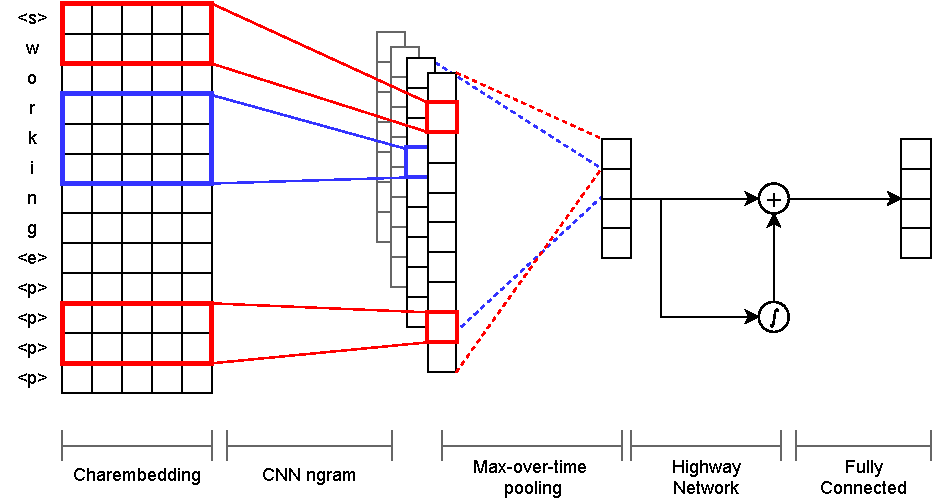
\includegraphics[width=.8\linewidth]{images/model2.pdf}
            \caption{OOV Inferencing Model}
            \label{fig:model}
        \end{figure}

        On figure \ref{fig:model}, starting and ending token is added
        at the beginning and the end of the word respectively.
        Furthermore, padding token is added if the input word is
        shorter than the length of the input size of the model. The
        padding token is a zero vector $\vec{0}$ and $\vec{0} * k =
        \vec{0}$ for any $k$. This is to ensure that part of input
        that got padded does not goes through maxpool layer since only
        grams that has highest value can goes through the next layer
        and minimum value of ReLU is 0.

    \subsection{Error and Backpropagation}
        The output of the neural network $\tilde{e}$ then compared
        with the original embedding $e$ to learn new parameters for
        the neural network using mean squared error function as shown
        on \ref{eq:errorf}

        \begin{equation}
            \label{eq:errorf}
            Error = \frac{1}{2} \Vert e - \tilde{e} \Vert ^{2}
        \end{equation}

        The error then backpropagated to fine-tune the neural network
        parameters.
        
\section{Measuring Performance on Downstream Tasks}
    In natural language modeling (NLP), there are several tasks that
    make used of word embedding. Hence that, the generated embeddings
    from the model can be evaluated by using those downstream tasks.
    The results then compared with the state-of-the-art OOV handling
    model \textsc{Mimick} \citep{mimicking2017Pinter}.
    
    \subsection{Part-of-Speech Tagging}
        Part-of-speech tagging or POS-tagging is a task of classifying
        usage of words in sentence or corpus based on the grammatical
        usage of the word \{cite\}, for example: verb, noun, adverb,
        etc. Given sentence $S = \{w \in \mathcal{V} \vert ((w_1,
        t_1), (w_2, t_2)\\, \dots, (w_n, t_n)\}$ with its POS-tag $t_i$,
        each word $w_i$ that exist in the vocabulary $w_i \in
        \mathcal{V}$ and $w_i \in S$ is transformed into embedding
        $e_i$. For the OOV, the sequence of the characters building a
        word transformed into sequence of character embedding
        $[\hat{g}]_i$ using model represented in equation
        \ref{eq:word2charemb} then the embedding $e_i$ is predicted
        using the OOV handling model.

        The sequence of embeddings $e_i$ then fed into bi-LSTM with
        logsoftmax activation function at the output to get the
        POS-tag. To ease up computation time, adaptive logsoftmax is
        used \citep{grave2018efficientsoftmax}. Instead of calculating
        the whole classification, the frequent and infrequent classes
        are separated thus there are many chance that only frequent
        classes needs to be calculated. The complete process of
        POS-tagging process is shown in figure \ref{fig:postag}. After
        training was done, the accuracy of the POS-tagger based on
        different OOV handling model were compared.

        \begin{figure}
            \centering
            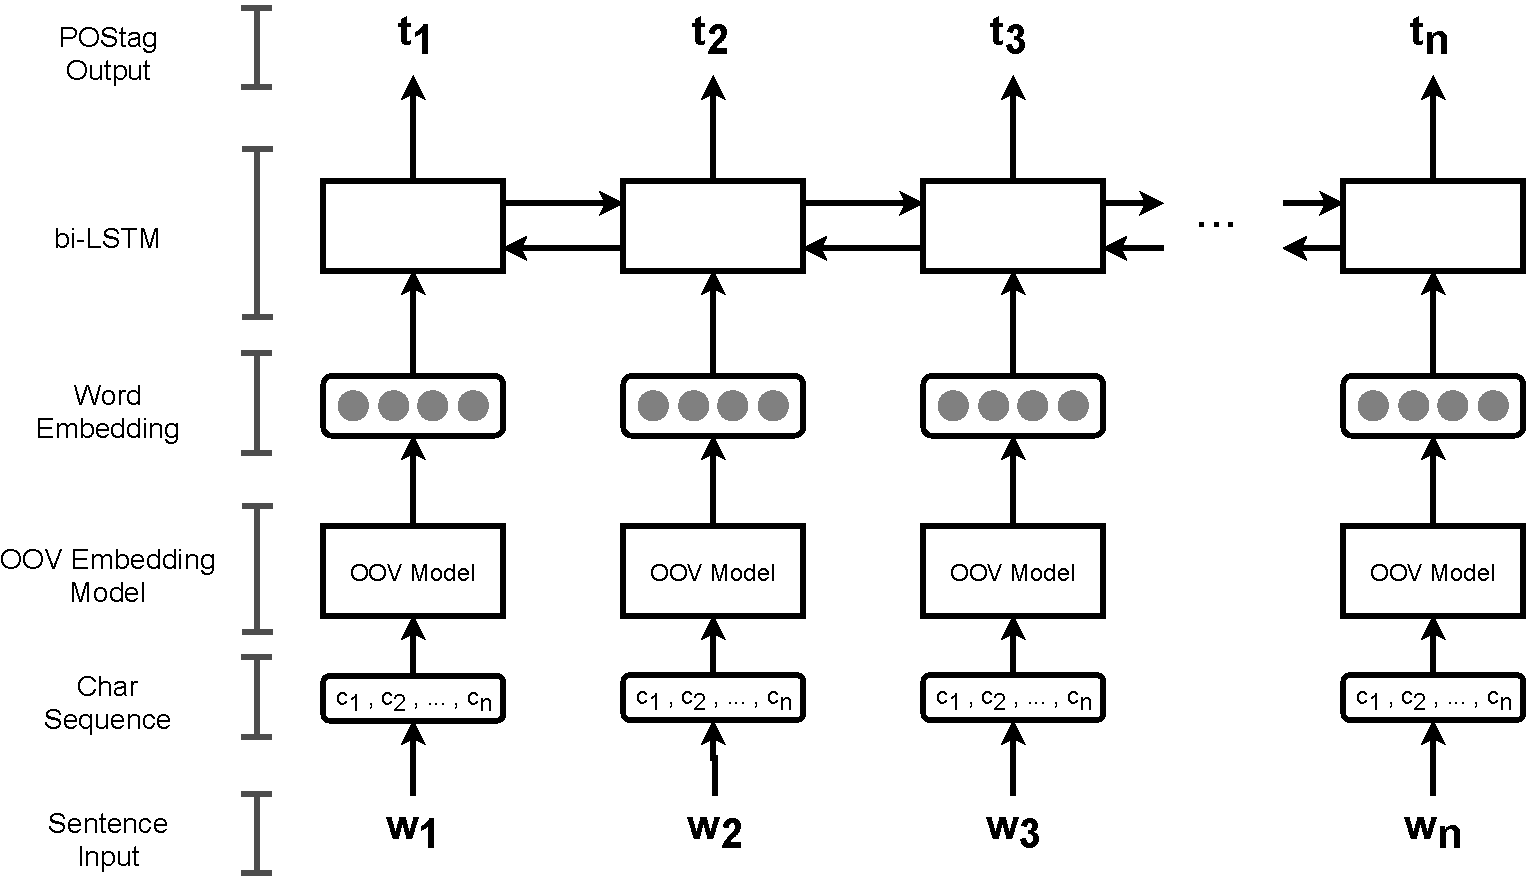
\includegraphics[width=.8\linewidth]{images/postag.pdf}
            \caption{Pos-tagging Process}
            \label{fig:postag}
        \end{figure}
 
    \subsection{Word Similarity Tasks}
        Word similarity tasks is basically task to evaluate the
        similarities between two words based on human given scores.
        Generally, several human subject were given pairs of words and
        asked to score its similarities. Those scores then will be
        used to determine the agreements between subjects that certain
        word pairs have stronger connection and the others are weaker.
        In order to calculate the agreements between the OOV generated
        embedding and the data that is scored by human, Spearman's
        rank correlation coefficient is used. Firstly, given a pair
        $(w_1, w_2)$, the cosine distance of the embedding $e_1$ and
        $e_2$ based on the generated OOV model for $w_1$ and $w_2$
        calculated respectively using equation \ref{eq:cosinesim}.

        \begin{equation}
            \label{eq:cosinesim}
            cosine\ similarity = \frac{e_1 \cdot e_2}{\Vert e_1 \Vert \Vert e_2 \Vert}
        \end{equation}

        After all of the cosine distance for all pairs are calculated,
        Spearman rank's correlation from the dataset and the generated
        embedding are calculated by using equation \ref{eq:spearman}
        and by using equation \ref{eq:spearmantied} when no tied ranks
        exists. The results of both \textsc{Mimick} and the proposed
        model from several word similarity datasets then averaged and
        compared.
        
        \begin{align}
            \label{eq:spearman}
            \rho    &= \ddfrac{n\sum_{i=1}^n u_i v_i - \Bigg( \sum_{i=1}^n u_i \Bigg) \Bigg( \sum_{i=1}^n v_i \Bigg)}{\sqrt{\Bigg[ n \sum_{i=1}^n u_i^2 - \Bigg( \sum_{i=1}^n u_i \Bigg)^2 \Bigg] \Bigg[ n \sum_{i=1}^n v_i^2 - \Bigg( \sum_{i=1}^n v_i \Bigg)^2 \Bigg] }}\\
            \label{eq:spearmantied}            
                    &= 1 - \ddfrac{6 \sum_{i=1}^n d_i^2}{n(n^2 - 1)}\ \text{where}\ d_i = u_i - v_i
        \end{align}
